\documentclass[twocolumn]{article}

\usepackage{amssymb}
\usepackage{amsmath}
\usepackage{graphicx}
\usepackage{epstopdf}
\usepackage{fancyhdr}
\usepackage{algpseudocode}

\DeclareMathSizes{36}{36}{36}{36}

\title{Massively Parallel Ant Colony Optimization Applied to the Traveling Salesman Problem}
\author{Forest Trimble, Scott Todd\\trimbf@rpi.edu, todds@rpi.edu}

\begin{document}

\maketitle

\pagestyle{fancy}
\fancyhead{}
\fancyhead[L]{Trimble, Todd}
\fancyhead[C]{Massively Parallel ACO on the TSP}
\fancyhead[R]{\today}


\begin{abstract}
  \emph{NP-complete problems have often fascinated programmers and mathematicians alike
  for their difficulty, and the traveling salesman problem is no exception. We 
  study ant colony optimization as applied to the traveling salesman problem, 
  and run and analyze its performance on the Blue Gene/Q. }
\end{abstract}

\section{Background}

\subsection{The Traveling Salesman Problem}

The Traveling salesman problem (TSP) is an extensively-studied NP-complete problem 
in theoretical computer science with varied applications throughout delivery, 
transportation, planning, and logistic operations. In the formulation of the 
problem, a list of cities is given and the distances between each pair of cities
is known. The question, then, is: what is the shortest possible path from city to
city that visits each city exactly once? In particular, we studied the symmetric
Traveling salesman problem, where the distance from any city A to any city B
is the same as the distance from city B to city A. In this case, the problem
can be modeled as an undirected graph, with vertices representing cities and
edges representing paths between cities. For interests' sake, Figure \ref{fig:opt2392}
shows an optimal tour of 2392 cities in the undirected case. \\

\begin{figure}
  \centering
  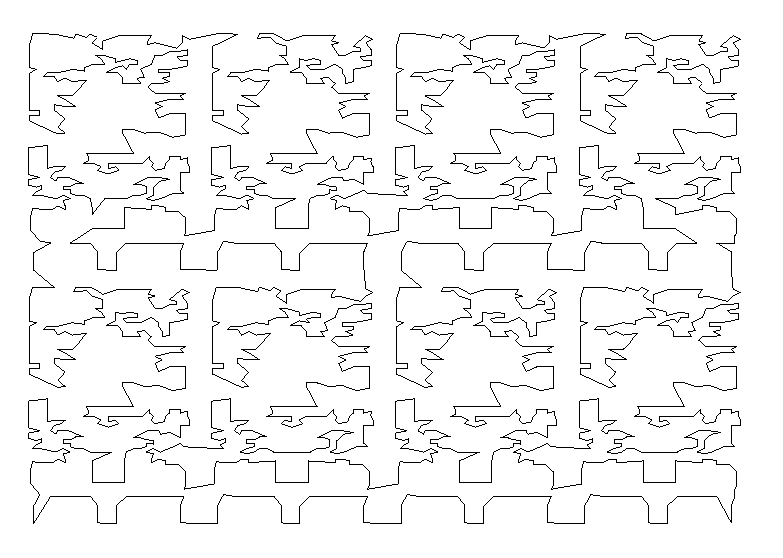
\includegraphics[height=2.2in]{plots/pr2392.eps}
  \caption{An Optimal TSP Tour of 2392 Cities} \label{fig:opt2392}
\end{figure}

The brute force approach to the TSP, which checks each possible solution, takes 
on the order of $\mathcal{O}(n!)$ time. Brute force is generally a pretty poor choice of
algorithm, and that is no different here: as it stands, the most efficient 
algorithms which provably return the optimal solution use dynamic
programming and operate in $\mathcal{O}(n^22^n)$ time and $\mathcal{O}(2^n)$ space. 
This is a massive time improvement, but it is still computationally intractable, as 
these large run-times and space requirements are prohibitively expensive even on 
supercomputer-class machines. Because of this, a large number of approximation 
algorithms have been formulated that are able to quickly approach the optimal 
solution, some provably within a certain threshold or with a high probability of
being particularly close to the optimal solution. 

\subsection{Ant Colony Optimization} 

The Ant Colony Optimization algorithm (ACO) for the Traveling salesman problem 
is one such approximation algorithm which lends itself well to parallel 
computation. It was first proposed by Marco Doringo's PhD thesis in 1992 \cite{dorigo}. 
Inspiration for this technique comes from the natural world, where ants in a
colony wander seemingly aimlessly until they come across food, leaving
a trail of pheromones for other ants to detect and follow. Pheromones
evaporate over time, so shorter paths accumulate pheromones in a higher density 
more reliably than longer paths. An emergent property of this behavior is that 
efficient paths to food sources will become apparent as more ants wander and 
follow these trails over time. Interestingly, the natural world provides a number
of such heuristics for optimization problems. \\

Just as these ants are able to find efficient routes to their food sources by
utilizing this emergent behavior, computers are able to find short paths through
graphs for the TSP by simulating ants and their pheromone trails. \\

An added advantage to the ACO, which we did not explore in our research, is that
the virtual ants are able to adapt to changes in their environment to 
dynamically adjust their preferred path around newly introduced obstacles \cite{iridia:aco}.

\section{Implementation} \label{sec:impl}

It is important to understand how ACO works before we dive into 
the details of our implementation. As such, section \ref{sub:aco} delves
into the concepts behind the ACO before we cover the
specifics of our implementation in section \ref{sub:acoimpl}

\subsection{Generalized ACO Algorithm} \label{sub:aco}

Ant Colony Optimization is a randomized process that uses a few things to aid
in its probabilistic selection:
\begin{itemize}
\item distances between cities
\item pheromone concentrations along edges ($\tau$)
\item heuristic parameters $\alpha$, $\beta$, and $\rho$
\end{itemize}
Basically, shorter distances and higher pheromone concentrations will
increase the probability that an ant will travel along an edge. The 
heuristic parameters allow for some variation as to how important 
each of these factors is. This is necessary because an effective 
implementation of the ACO for TSP algorithm must balance the tendency
for ants to follow efficient paths with the desire to discover new, 
perhaps more efficient paths. If the simulated ants follow the 
pheromone trails too closely, they may quickly get caught in local
minima. \\

The heuristic parameters $\alpha$ and $\beta$ are weights for the distances and 
the pheromones, respectively, and they can be chosen to help avoid this. They 
are used to calculate the probability, $p^k_{ij}$, of an ant following an edge
$ij$ at iteration $k$ according to 
\begin{equation}
p_{ij}^k = \frac{(\tau^k_{ij})^\alpha(d(C_i,C_j)^-\beta)}{\sum_{i=1}^m 
  (\tau^k_{ij})^\alpha(d(C_i,C_j)^{-\beta})} \label{eq:probs}
\end{equation}
Thus, if $\alpha >> \beta$, the pheromones will factor in far more than the
distances. When $\beta >> \alpha$, the same is true only if the distances are 
normalized to the range $[0,1]$; otherwise $\|\beta\|$ is effective only in 
weeding out the larger distances. Some researchers have experimented with 
updating the heuristic parameters as the algorithm executes \cite{ipcsit:aco}.\\

The final heuristic parameter, $\rho$, is used to 
determine how quickly pheromones decay. This is required to ensure that the pheromones do not
drastically overtake the distances in importance and that paths that are not used become 
progressively less and less attractive. Pheromone concentration is calculated as follows:
\begin{equation}
\tau^k_{ij} = \rho \tau^{k-1}_{ij} + \Delta \tau^k_{ij}, \label{eq:phers}
\end{equation}

which means that the base amount will decay by a factor of $\rho$ and each ant
that uses that edge will deposit some $\Delta\tau^k_{ij}$ amount of pheromone on
that edge. In many implementations of this algorithm, the $\Delta\tau^k_{ij}$
value is proportional to the path length traveled by ant $k$ \cite{iridia:aco} 
\cite{ipcsit:aco} \cite{jungblut:aco}. \\ 

Given this background, it becomes fairly simple to write out a general 
formula. The algorithm requires a set of $m$ cities, $C$. Given this, 
it repeatedly finds a tour through all the cities, beginning at a random city
(this is important) and selecting the next city by ``rolling the dice'' and
using \eqref{eq:probs} to select the edge. After a tour is found, the 
pheromones are updated. It is important that the starting city is random 
because this helps to avoid an overly greedy strategy. What follows is a
precise definition of the algorithm. \\

\noindent {\bf The Ant Colony Optimization Algorithm}
\begin{algorithmic}
  \State Given $C, \rho \in (0,1), \alpha > 0, \beta > 0$, where $|C| = m$
  \State Let $\tau$ be an $m \times m$ matrix of ones.
  \State $d = \infty$
  \For{$k = 0,1,2,\ldots $}
    \State Let $C_i = C_{\mbox{{\tiny BEGIN}}}\in C$ randomly
    \State $V = \{ C_i \}$
    \State $d_k = 0$
    \State $\tau_{ij} = \rho \tau_{ij}$
    \While {$V \not = C$}
       \State Let $p \in (0,1)$ randomly
       \State $\displaystyle p_j = \frac{(\tau_{ij}^\alpha)(d(C_i,C_j)^{-\beta})}{\sum_{n=1}^m 
         (\tau_{in}^\alpha) (d(C_i,C_n)^{-\beta})}$
       \State Set $j \in \mathbb{Z}$ s.t. $\displaystyle \sum_{n=1}^j p_n > p$ and 
       $\displaystyle \sum_{n=1}^{j-1} p_n < p$
       \State $\tau_{ij} = \tau_{ij} + d(C_i,C_j)^{-\beta}$
       \State $d_k = d_k + d(C_i,C_j)$.
       \State $V = V \cup C_j$
       \State $i = j$
    \EndWhile
    \State $d_k = d_k + d(C_i,C_{\mbox{{\tiny BEGIN}}})$
    \State $d = \min (d_k, d)$
  \EndFor \\
\end{algorithmic}

This algorithm is lacking in a few respects. First and foremost, end conditions are not present:
in this form it is designed to be run forever, acquiring a better solution (hopefully) at each
iteration. However, this is not how the algorithm is designed to be used, as the idea is to find
a quick solution that is ``close enough.'' Second, $\rho$, $\alpha$, and $\beta$ are left 
arbitrary. These parameters are heuristics: they must be found empirically, and there is much 
debate as to how to use them properly. These issues are discussed in section \ref{sub:acoimpl}.
Finally, this algorithm is not parallel; that is discussed in section \ref{sec:parallel}. 

\subsection{ACO on the TSP Implementation} \label{sub:acoimpl}



\section{Parallel Implementation} \label{sec:parallel}

\subsection{Parallelizing the Algorithm}

The algorithm lends itself to parallel execution. Indeed, each processor can
represent a single ant. On the small partition of the Blue Gene/Q that is
available, this yields 1024 ants scurrying around trying to find an optimal
TSP path, a veritable colony! Each processor can compute individual tours by
itself, but the parallel aspect comes into play when handling the pheromones.
In order for algorithm to work successfully, the pheromones need to come from 
all of the ants depositing their pheromones on their trail. Thus, an up-to-date
pheromone matrix is required. \\

However, keeping this available at all times is
very resource intensive. The challenge was to balance the algorithm's requirement
of the pheromones with computational resources. Initially, the solution was to
simply allreduce the matrix after each tour, but this became incredibly 
slow as processors scaled out. In order to combat this, the new solution was
to use a hybrid threading/parallel approach. Since eight threads per task has 
proven success on the Blue Gene/Q as an optimal configuration \cite{lolours},
that was the chosen setup. Leveraging the shared memory of threads cut the 
number of allreduces by a factor of eight (although the shared memory overhead
cut into the performance gains), but there was still room for improvement. Each
task now had a ``sub-colony'' of ants working together to find an optimal 
solution, and letting these small groups work on their own for a bit would allow
for slightly more deviation from the norm. Thus, the next step was to have 
each processor attempt to find some number of paths before updating to the global 
pheromone matrix. 

\section{Related Work}

Ivan Brezina Jr. and Zuzana \v{C}i\v{c}kov\'{a} \cite{mis:aco} studied the 
impact of the various control parameters on the quality of the solutions 
produced for the ACO for TSP algorithm. They found that with $\alpha=1$ and 
$\beta=5$, 10000 ants were able to approximate the optimal solution to a 32 city
problem within 0.83\% over 242 iterations. \\

Marco Dorigo and Luca Maria Gambardella \cite{iridia:aco} modelled local and 
global pheromone trails in their implementation of the ACO for TSP algorithm. 
The global pheromone trail was updated by only the ant with the shortest tour. 
The local pheromone trails were motivated by trail evaporation and were designed
to avoid all ants choosing a very strong edge. They found their algorithm was 
able to find good solutions to the TSP for both symmetric and asymmetric graphs.
They also indicated a few techniques that could be employed to improve upon the 
algorithm in the future, including local optimization heuristics where each ant 
would arrive at a local maximum before updating the trail and parallelizing the
algorithm. \\

Daniel Kunkle and Stephen Guerin released a video \cite{youtube:aco}
demonstrating an interactive TSP solver using the ACO. \\

Zar Chi Su Su Hlaing and May Aye Khine \cite{ipcsit:aco} expanded on the basic 
ACO algorithm by strategically distributing ants and monitoring information 
entropy to update the heuristic parameters as the simulation progressed. 
Compared to other optimizations, such as control of search construction and 
partitioned groups of ants, they found that their proposed algorithm had the 
potential to greatly increase the convergence speed of the ACO algorithm. \\

Thomas Jungblut details his multithreaded Java implementation of the ACO for TSP
algorithm in a blog post \cite{jungblut:aco}. He found the best results to a 52
city problem using $\alpha=-0.2$ and $\beta=9.6$ with 40960 worker ants.

\section{Performance Results}

We obtained data sets for the TSP from TSPLIB \cite{tsplib}, since the problems
there are accompanied by optimal solutions calculated using exact methods that
we would be able to compare our results with. 

We performed a strong scaling study, where the problem size remained constant
while the processor count increased.\\


\section{Analysis of Performance Results}

\begin{figure}
  \centering
  \includegraphics[height=2.2in]{plots/data_dist.eps}
  \caption{Distances found in a strong scaling study}
\end{figure}

\begin{figure}
  \centering
  \includegraphics[height=2.2in]{plots/data_time.eps}
  \caption{Time taken in a strong scaling study}
\end{figure}

\begin{figure}
  \centering
  \includegraphics[height=2.2in]{plots/data_tour.eps}
  \includegraphics[height=2.2in]{plots/opt_tour.eps}
  \caption{An ACO tour (top) and the Optimal Tour (bottom) for a 150 city TSP}
\end{figure}

big words go here..\\


\section{Summary and Future Work}

optimistic words and lofty goals go here...\\

\section{Team Member Contributions}

\noindent Forest Trimble coded out and wrote up the actual algorithm. He was 
responsible for writing a good chunk of the write-up. \\

\noindent Scott Todd set up the base of the code structure, including the input
file parsing and parameter initialization. He prepared input files and testing
materials. He performed the initial research and wrote the first draft for the
background write-up.

\nocite{*}
\bibliographystyle{plain}
\bibliography{findings}
\end{document}
